% ОПЫТ №24 Закон сохранения момента количества движения. Скамья Жуковского
\sloppy
\documentclass[14pt,a4paper,oneside]{extarticle}	% Размер основного шрифта и формата листа
\usepackage{xltxtra}						% Используется для вывода логотипа XeLaTeX
\usepackage{xunicode}						% Кодировка документа
\usepackage{polyglossia}					% Загружает пакет многоязыковой верстки
\newfontfamily\russianfont{Book Antiqua}
%\setmainfont{Liberation Serif}						% Основной шрифт текста
\setmainfont{Book Antiqua}
\setdefaultlanguage{russian}				% Основной язык текста
\setotherlanguage{english}					% Дополнительный язык текста
\linespread{1}							% Межстрочный интервал выбран 1
\usepackage[left=2.5cm,
right=1.5cm,vmargin=2.5cm]{geometry} % Отступы по краям листа
\bibliographystyle{ugost2008}

\usepackage{xcolor}
\usepackage{hyperref}
% Цвета для гиперссылок
\definecolor{linkcolor}{HTML}{359B08} % цвет ссылок
\definecolor{urlcolor}{HTML}{799B03} % цвет гиперссылок
\hypersetup{pdfstartview=FitH,  linkcolor=linkcolor,urlcolor=urlcolor, colorlinks=true}


%---------------------------%
%---- Пакеты расширений ----%
%---------------------------%

\usepackage{verbatim,indentfirst}
\usepackage{cite,enumerate,float}
\usepackage{amsmath,amssymb,amsthm,amsfonts}


%---------------------------%
%--- Вставка иллюстраций ---%
%---------------------------%
\usepackage{graphicx}
\usepackage{subfigure}
%\graphicspath{{Images/}}
\usepackage{fontspec}
\usepackage{bm}

\begin{document}
%		\pagestyle{empty} %  выключаенм нумерацию
%\setcounter{page}{3}% Нумерация начинается с третьей страницы
%\renewcommand{\contentsname}{\center{Содержание}}
%\tableofcontents
	
	\newpage
	\begin{center}
		%\addcontentsline{toc}{section}{Опыт 16. Нахождение центра масс}
		\subsection*{Скамья Жуковского}
	\end{center}
		
\begin{figure}[H] 	
	\centering 	
	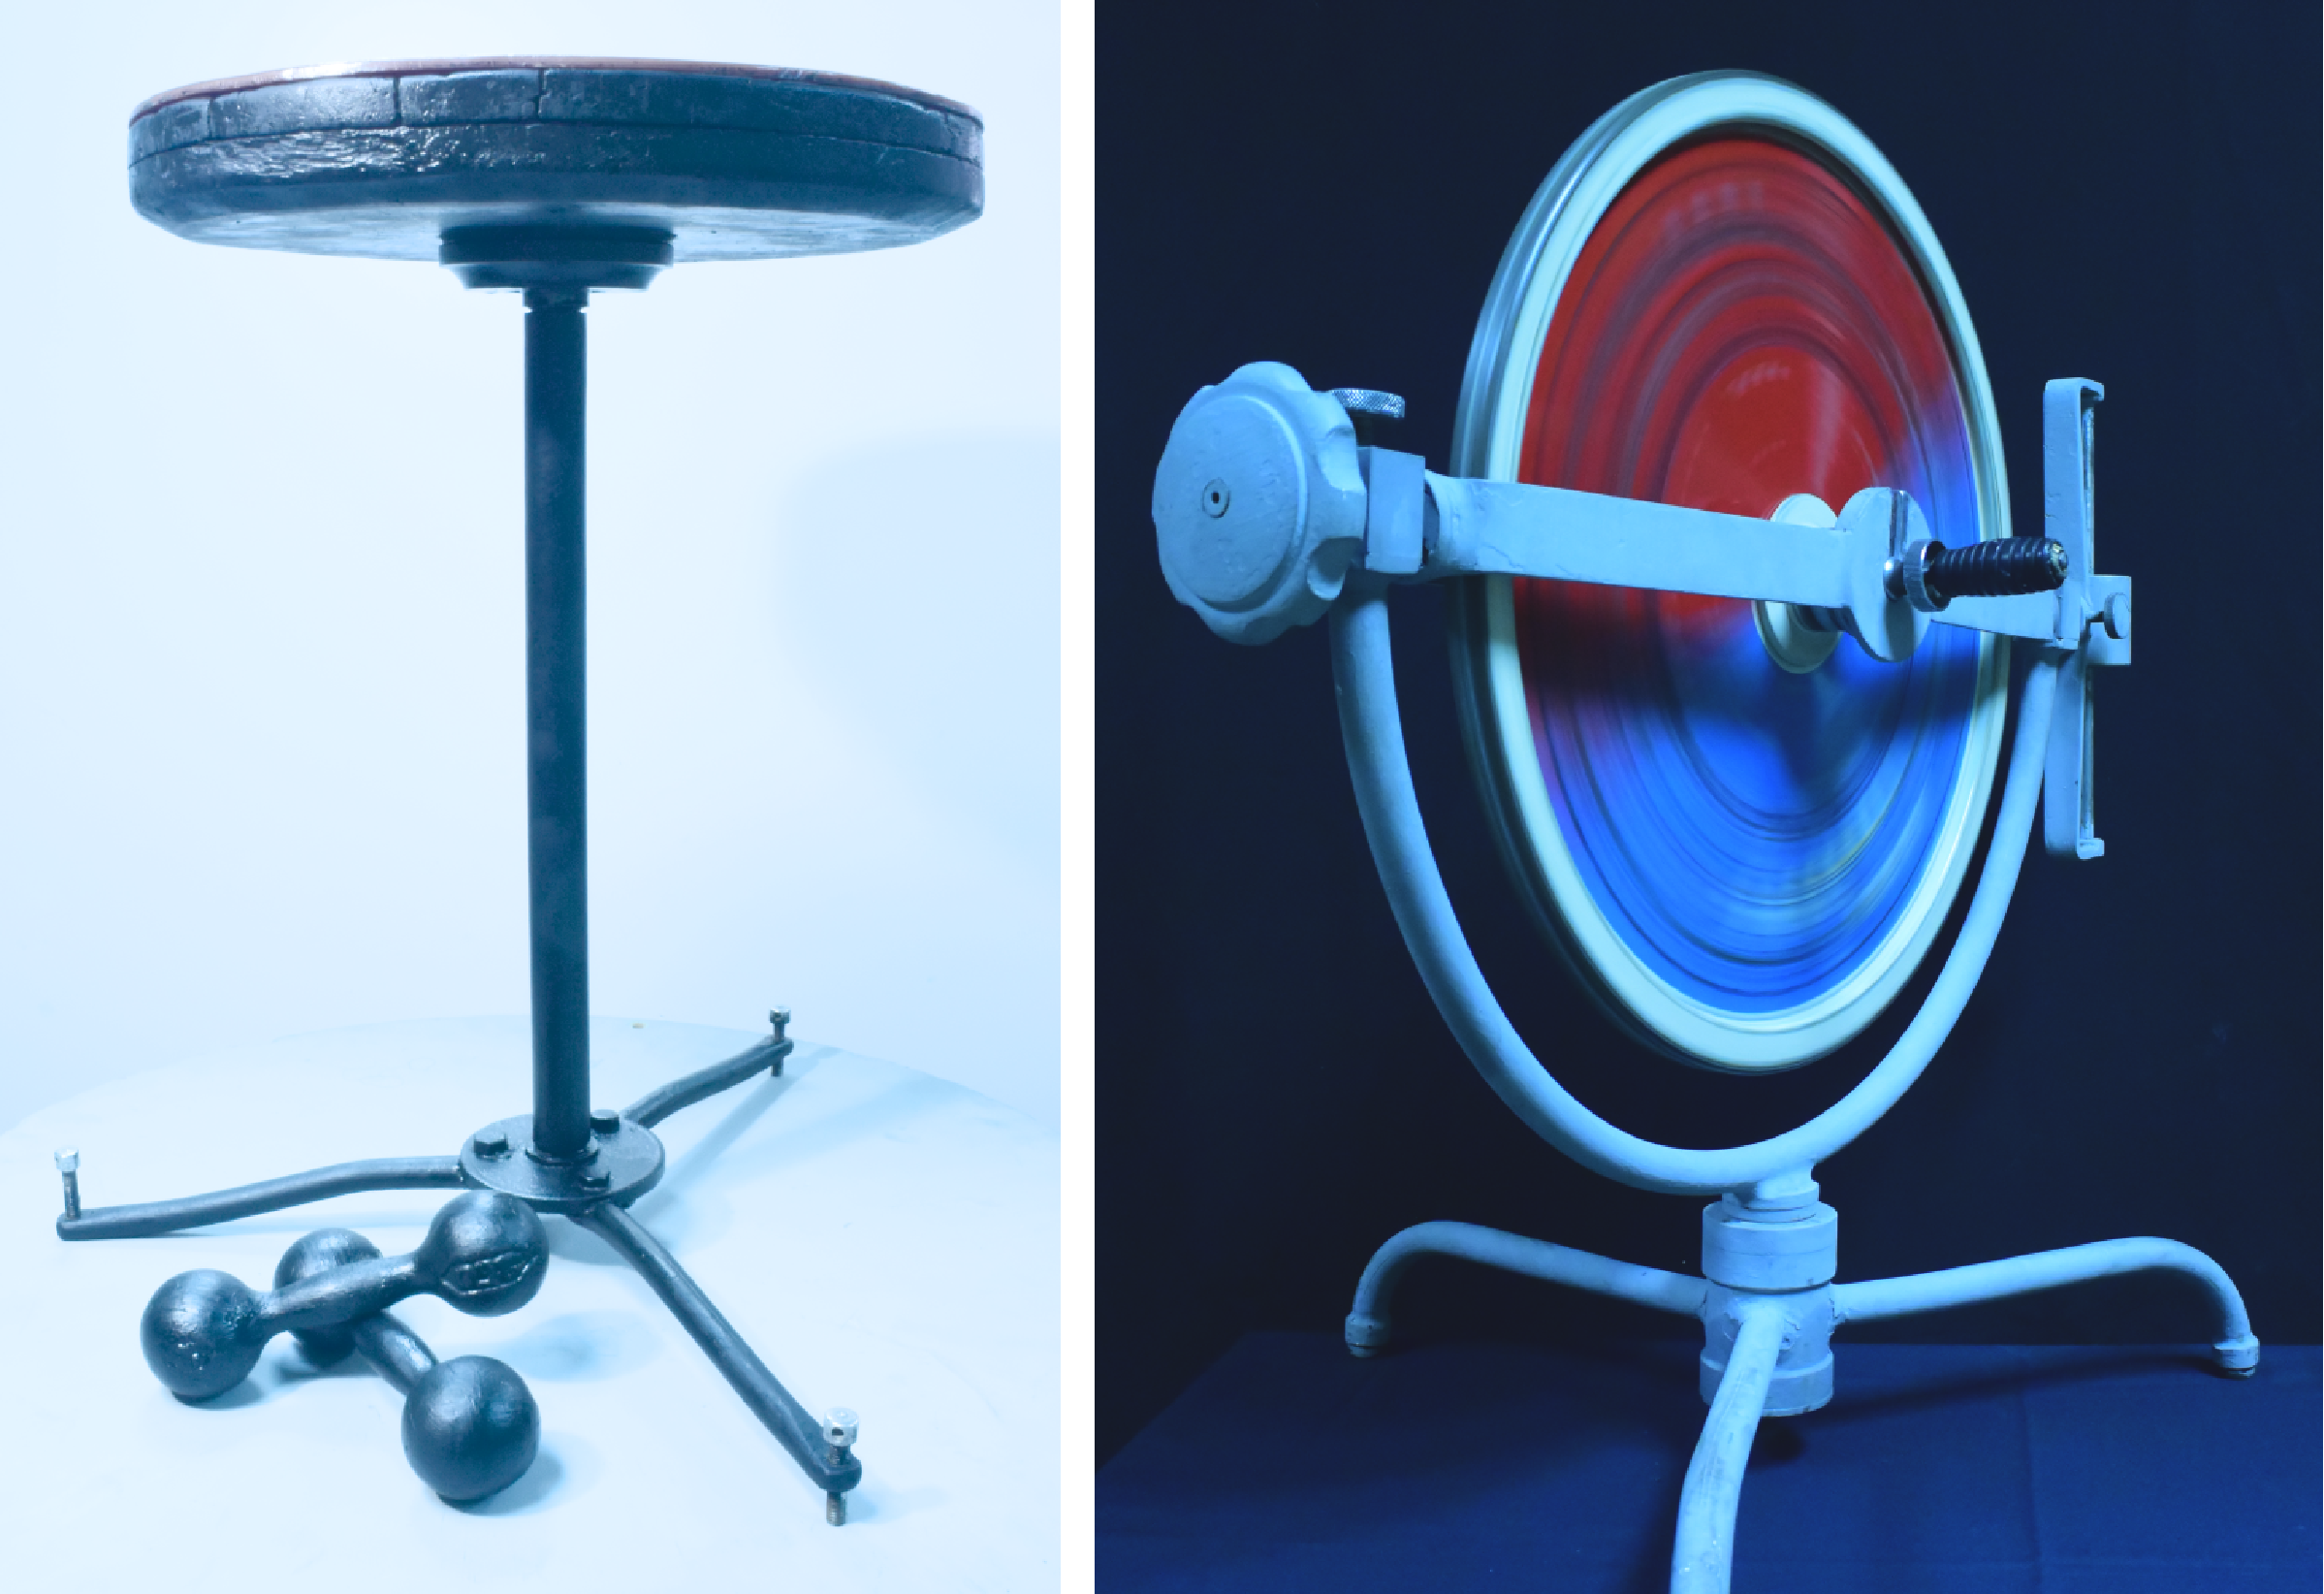
\includegraphics[width=0.9\linewidth]{chair-1.png}
	\caption{Демонстрация закона сохранения момента импульса в опытах со скамьей Жуковского}
	\label{chair-1}
\end{figure}
	
	\subsection*{\underline{Оборудование:}}

			\begin{enumerate} 
			\item Скамья Жуковского (вращающаяся платформа).
			\item Два груза массой 250 г каждый.
			\item Гироскоп в кардановом подвесе.
		\end{enumerate}

\subsection*{\underline{Основные определения:}}
	
	Момент импульса — одна из мер механического движения материальной точки или системы.
	Особенно важную роль момент импульса играет при изучении вращательного движения.
	Как и для момента силы, различают момент импульса относительно центра (точки) и относительно оси. 
	Для вычисления момента импульса \textbf{L} материальной точки относительно центра \textit{О} или оси \textit{z} справедливы те же формулы, что и для вычисления момента силы, если в них заменить вектор силы \textbf{F} вектором импульса \textit{m}\textbf{v}.
	Таким образом, $\textbf{L} = \textbf{r}\times (m\textbf{v})$, где \textbf{r} — радиус-вектор движущейся точки, проведенный из центра \textit{О}.
	
	Изменение момента импульса точки происходит под действием момента $ \textbf{М}_F $ приложенной силы и определяется теоремой об изменении момента импульса (уравнением моментов), выражаемой уравнением
	$$ \frac{\Delta \textbf{L}}{\Delta t}  = \textbf{М}_F.$$
	
	Главный (полный) момент импульса механической системы относительно центра \textit{О} или оси \textit{z} равен соответственно геометрической или алгебраической сумме моментов импульса всех точек системы относительно того же центра или оси, т. е. $ \textbf{L} = \sum \textbf{L}_i $. 
	Вектор \textbf{L} может быть определен его проекциями $ L_x $, $ L_y $, $ L_z $ на соответсвющие координатные оси выбранной прямоугольной системы координат.
	Если ось \textit{z} является главной осью инерции для начала координат \textit{О}, то $ L_z = I_z\omega $.
	
	Изменение главного момента импульса системы происходит под действием только внешних сил и зависит от их главного момента $ \textbf{M}^\text{внеш} $.
	Эта зависимость определяется теоремой об изменении полного момента импульса системы, выражаемой уравнением (уравнением моментов для системы точек) $$ \frac{\Delta \textbf{L}}{\Delta t} = \textbf{M}^\text{внеш}.$$
	Аналогичным уравнением связаны моменты $ L_z $ и $ M_z^\text{внеш} $.
	Если $ \textbf{M}^\text{внеш}=0 $ или $ M_z^\text{внеш}=0 $, то соответственно \textbf{L} или $ L_z $ будут величинами постоянными, т. е. имеет место закон сохранения момента импульса.
	Таким образом, внутренние силы не могут изменить полный момент импульса системы, но момент импульса отдельных частей системы или угловые скорости под действием этих сил могут изменяться.
	
У вращающегося вокруг вертикальной оси \textit{z} фигуриста (или балерины) величина $ L_z = I_z\omega $ будет постоянной, т. к. практически $ M_z^\text{внеш}=0 $.
	Но изменяя движением рук или ног значение момента инерции $ I_z $, он может изменять угловую скорость $ \omega $.
	
	Другим примером выполнения закона сохранения момента импульса служит появление реактивного момента у двигателя с вращающимся валом (ротором).
	Понятие о моменте импульса широко используется в динамике твердого тела, особенно в теории гироскопа.
		
	\subsection*{\underline{Краткое описание:}}
	
Скамья Жуковского состоит из станины с опорным шариковым подшипником, в котором вращается верхняя часть скамьи с горизонтальной круглой платформой.
Центр платформы совпадает с осью вращения скамьи.
		
	\textit{Опыт 1}:
Взяв в каждую руку груз массой около 250 г, человек садится на скамью и разводит руки в стороны.
Второй человек «раскручивает» скамью так, чтобы она и сидящей на ней человек вращались со скоростью приблизительно один оборот в 1.5-2 секунды, и отходит в сторону. 
Сидящий на скамье человек резким движением приближает руки с грузом к груди, уменьшая свой момент инерции.
Так как произведение момента инерции на угловую скорость в замкнутой системе остается постоянным, то платформа с сидящим на ней человеком начинает вращаться значительно быстрее. 
Разведя руки с грузами в стороны для увеличения момента инерции, он вновь уменьшает свою скорость вращения.
Демонстрацию следует повторить несколько раз.

\textit{Опыт 2}:
Возьмем колесо или деревянный круг и вставим в его втулку ось.
Возьмемся за ось двумя руками по разные стороны от колеса, и попробуем повернуть ее в вертикальной плоскости.
Оказывается, что сделать это довольно легко, так как невращающееся колесо не оказывает этому повороту никакого сопротивления. Придадим теперь колесу быстрое вращение вокруг его собственной оси с угловой скоростью омега и вновь попытаемся повернуть его в вертикальной плоскости. В ходе опыта можно заметить, что ось колеса, сопротивляясь этому повороту, поворачивается вместе с тем в горизонтальной плоскости.

\textit{Опыт 3}: Другой вариант демонстрации закона сохранения момента импульса показывают с использованием колеса с шариковым подшипником (от гироскопа в кардановым подвесе, масса которого в основном сосредоточена на периферии. 
Из-за того, что вся масса колеса сосредоточена на ободе, это колесо при быстром вращении обладает большим моментом инерции.
Раскрутив колесо и держа его ось горизонтально, это колесо передается в руки сидящему на скамье человеку.

Демонстратор (человек, который сидит на скамье) поворачивает ось вращающегося колеса так, чтобы она заняла вертикальное положение. 
Теперь момент импульса колеса относительно вертикальной оси не равен нулю, но общий момент системы относительно этой оси должен по-прежнему оставаться равным нулю; поэтому скамья с сидящим на ней человеком начинает вращаться в сторону, противоположную направлению вращения колеса.
Если повернуть ось колеса на 180°, то скамья изменит направление вращения на противоположное.
В этом положении общий момент импульса системы относительно вертикальной оси равен нулю (в начале опыта ось вращения колеса  горизонтальна).
	
	\subsection*{\underline{Теория:}}
	
\textit{Опыт 1}:
 Человек, держащий гири составляет вместе со скамьей замкнутую механическую систему, поэтому момент импульса $ I\bm{\omega} $ этой системы должен иметь постоянное значение.
 	\begin{figure}[H] 	
 	\centering 	
 	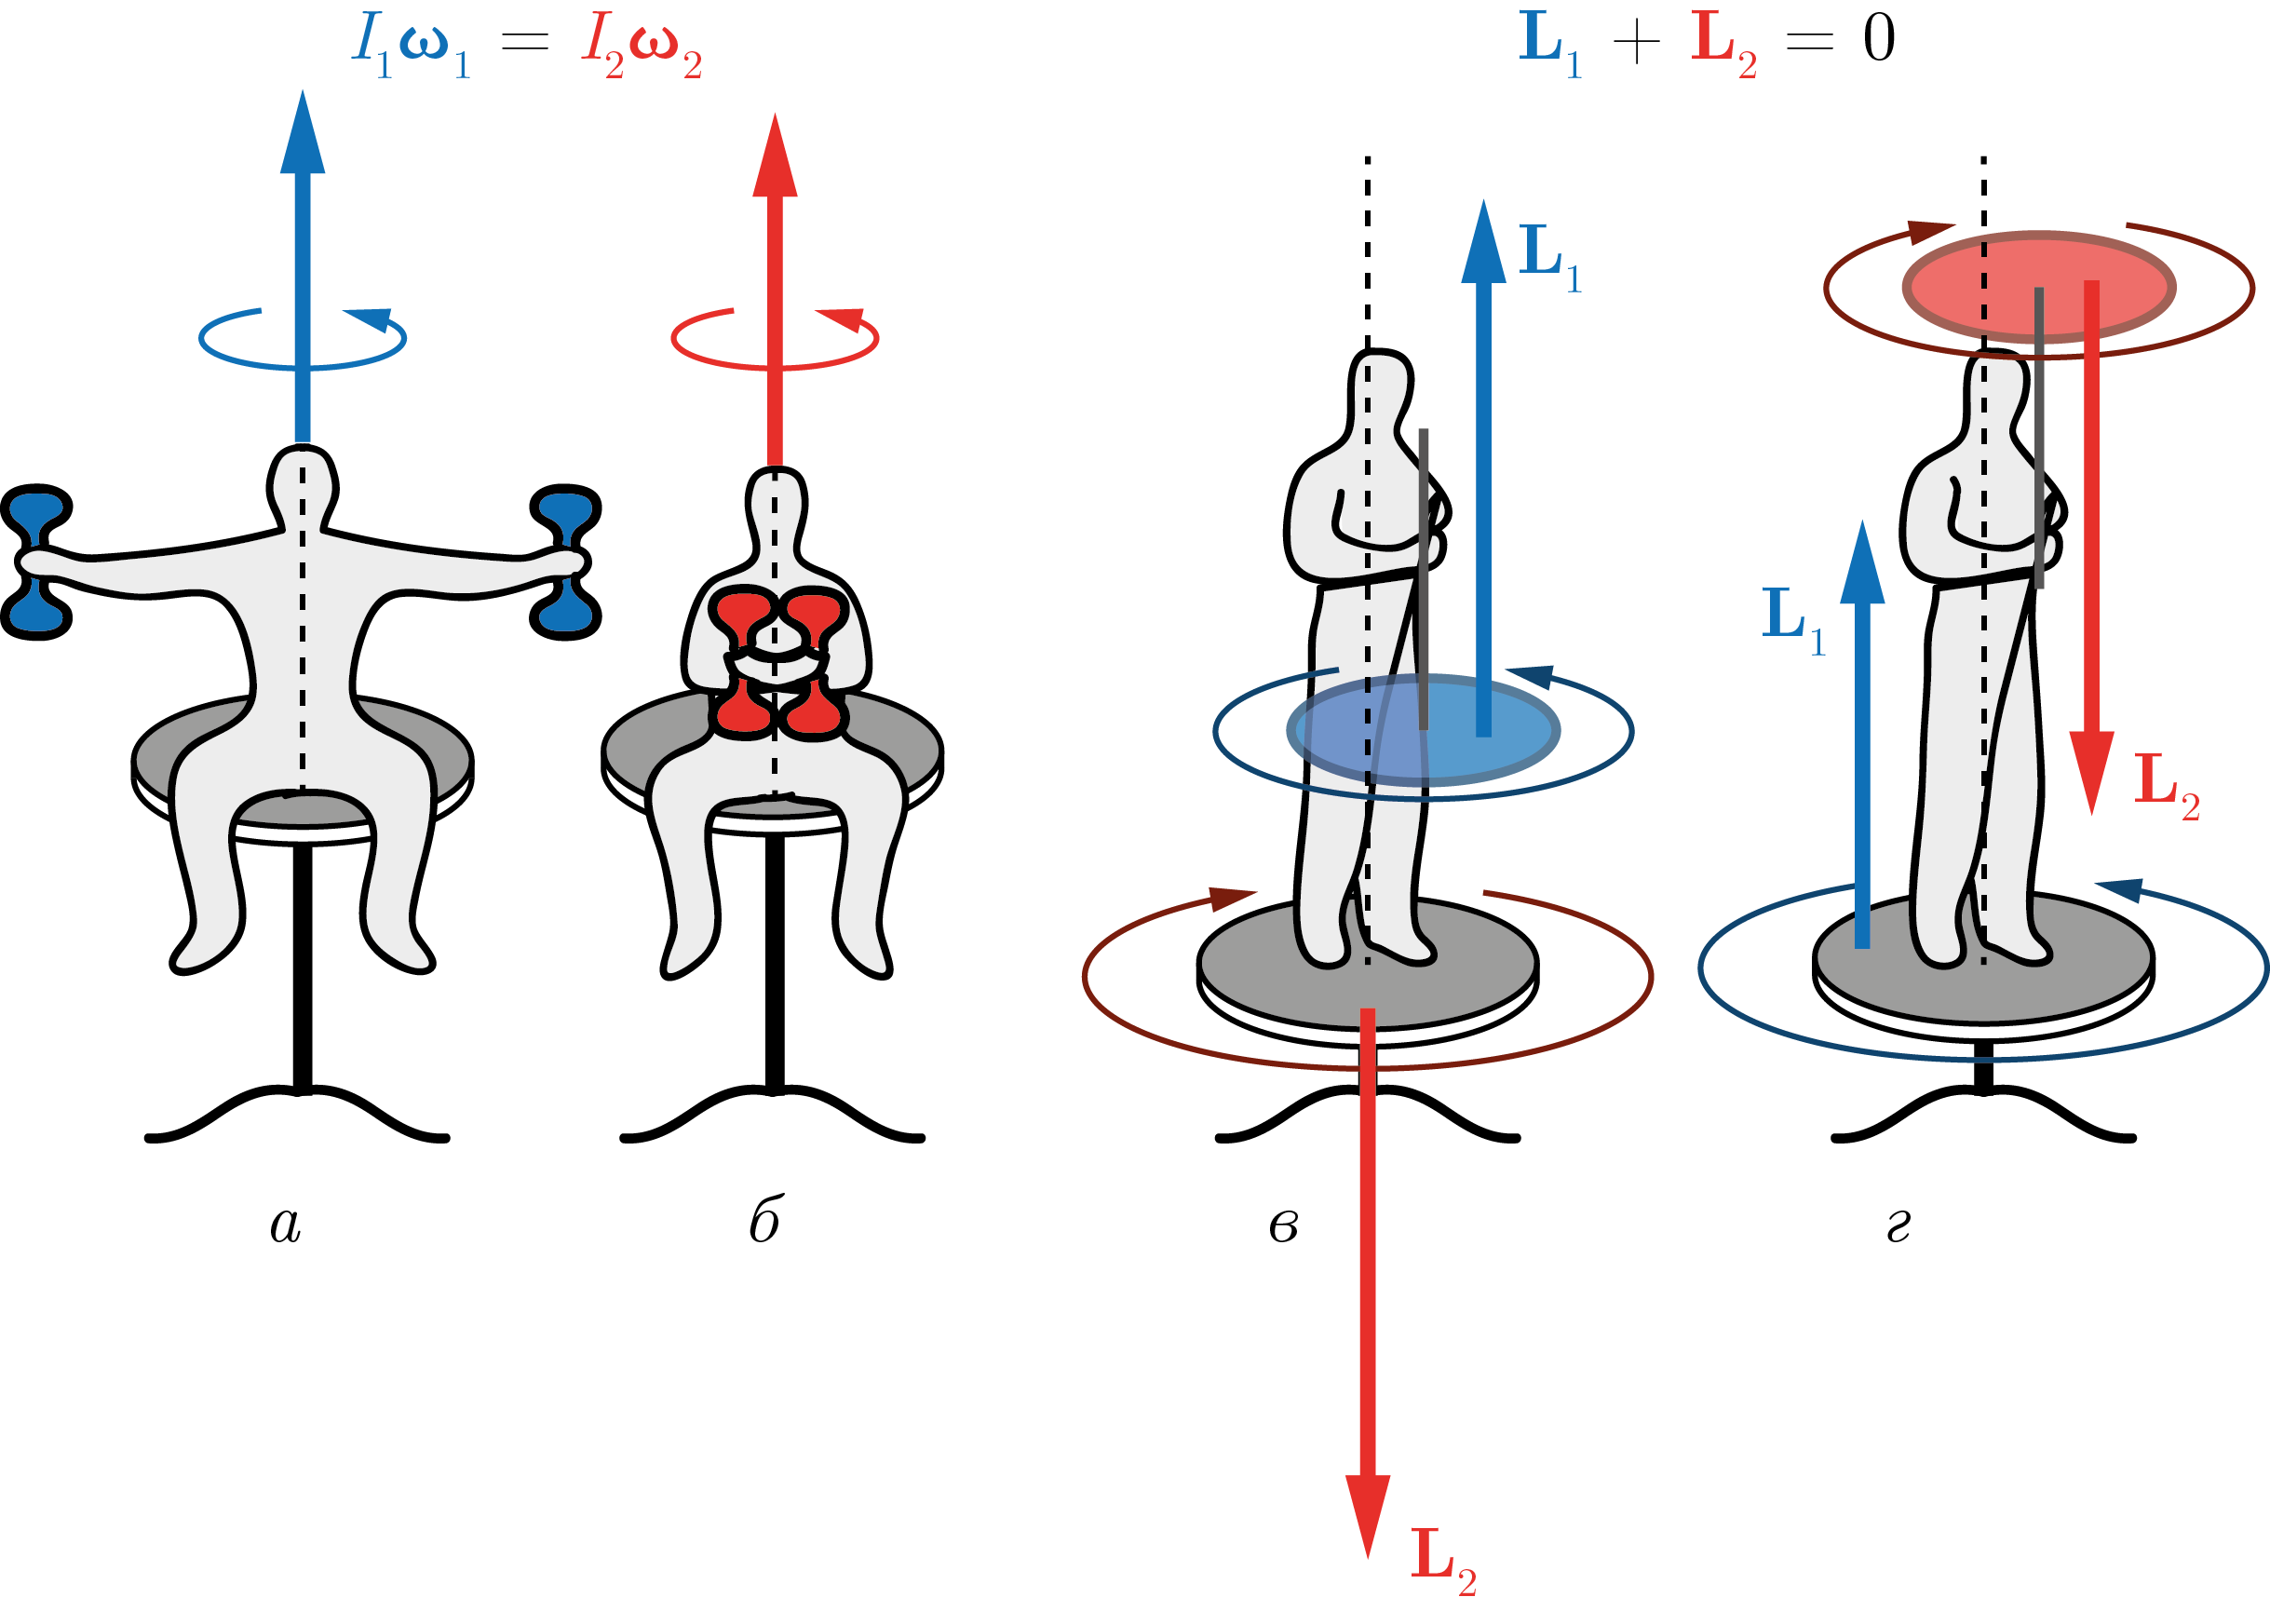
\includegraphics[width=0.9\linewidth]{chair-2.png}
 	\caption{При изменении момента инерции системы за счет премещения рук или поворота гироскопа угловая скорость вращения скамьи Жуковского изменяется таким образом, чтобы полный момент импульса в системе остался равным начальному}
 	\label{chair-2}
 \end{figure}

 Следовательно для данного случая:
 \begin{equation}\label{chair-eq1}
 I_{1}\bm{\omega}_{1} =  I_{2}\bm{\omega}_{2},
 \end{equation} 
 где $ I_{1}  $ — момент инерции человека с вытянутыми руками, находящегося на скамье (\ref{chair-2},\textit{а}), $ I_{2}  $ — момент инерции человека с прижатыми к груди руками (\ref{chair-2},\textit{б}), $ \bm{\omega}_{1} $ — угловая скорость человека с вытянутыми руками (\ref{chair-2},\textit{а}), а $ \bm{\omega}_{2}  $ — момент инерции человека с прижатыми к груди руками (\ref{chair-2},\textit{б}).
 Выразив $ \bm{\omega}_{2} $:
 \begin{equation}\label{chair-eq2}
 \bm{\omega}_{2} =  \frac{I_{1}}{I_{2}}\bm{\omega}_{1},
 \end{equation}
 Угловую скорость можно выразить, через частоту вращения соотношением $ \bm{\omega} = 2\pi \nu  $.
 Произведя замену в уравнении (\ref{chair-eq2}) получим:
 \begin{equation}\label{chair-eq3}
 2\pi \bm{\nu}_{2} = 2\pi \frac{I_{1}}{I_{2}}\bm{\nu}_{1}.
 \end{equation}
 Сократив $  2\pi $ в выражении (\ref{chair-eq2}) получаем:
 \begin{equation}\label{chair-eq4}
 \bm{\nu}_{2} = \frac{I_{1}}{I_{2}}\bm{\nu}_{1}.
 \end{equation}
Момент инерции рассматриваемой системы, равен сумме моментов инерции тела человека $ I_{0} $ и момента инерции гирь в руках человека. Так как размер гирь много меньше расстояния их от оси вращения, то момент инерции гирь можно определить по формуле момента инерции материальной точки: $ I = mr^{2} $.
Следовательно,
\begin{equation}\label{chair-eq5}
I_{1} = I_{0} + 2m \left(\frac{l_{1}}{2} \right)^{2}.
\end{equation}
\begin{equation}\label{chair-eq6}
I_{2} = I_{0} + 2m \left(\frac{l_{2}}{2} \right)^{2} ,
\end{equation}
где $ m $ - масса каждой гири; $ l_{1} $ и $ l_{2} $ - первоначальное и конечное  расстояние между гирями.
Подставив выражение  (\ref{chair-eq5}) и  (\ref{chair-eq6}) в уравнение (\ref{chair-eq4}) получим:
\begin{equation}\label{chair-eq7}
I_{2} =  \frac{I_{0} + 2m \left(\frac{l_{1}}{2} \right)^{2}}{I_{0} + 2m \left(\frac{l_{2}}{2} \right)^{2}}\bm{\nu}_{1}.
\end{equation}
Из формулы  (\ref{chair-eq5}) и  (\ref{chair-eq6}) видно, что момент инерции зависит от положения грузов. 
При положении гирь на вытянутых руках $ (l_{1}) $ он оказывается больше, нежели при гирях прижатых к телу $ (l_{2}) $.
Оказывается, что $ I_{1} > I_{2} $, это и приводит к увеличению скорости вращения (\ref{chair-eq2}).
\newpage

\textit{Опыт 2}:
Объяснить причину сопротивления вращающегося колеса изменению его ориентации в пространстве довольно легко.
Действительно, стремясь повернуть ось колеса в вертикальной плоскости, демонстратор тем самым прикладывает к этой оси пару сил, момент \textbf{М} которой направлен вдоль оси \textit{y} (рис.\ref{chair-3}).
	\begin{figure}[H] 	
	\centering 	
	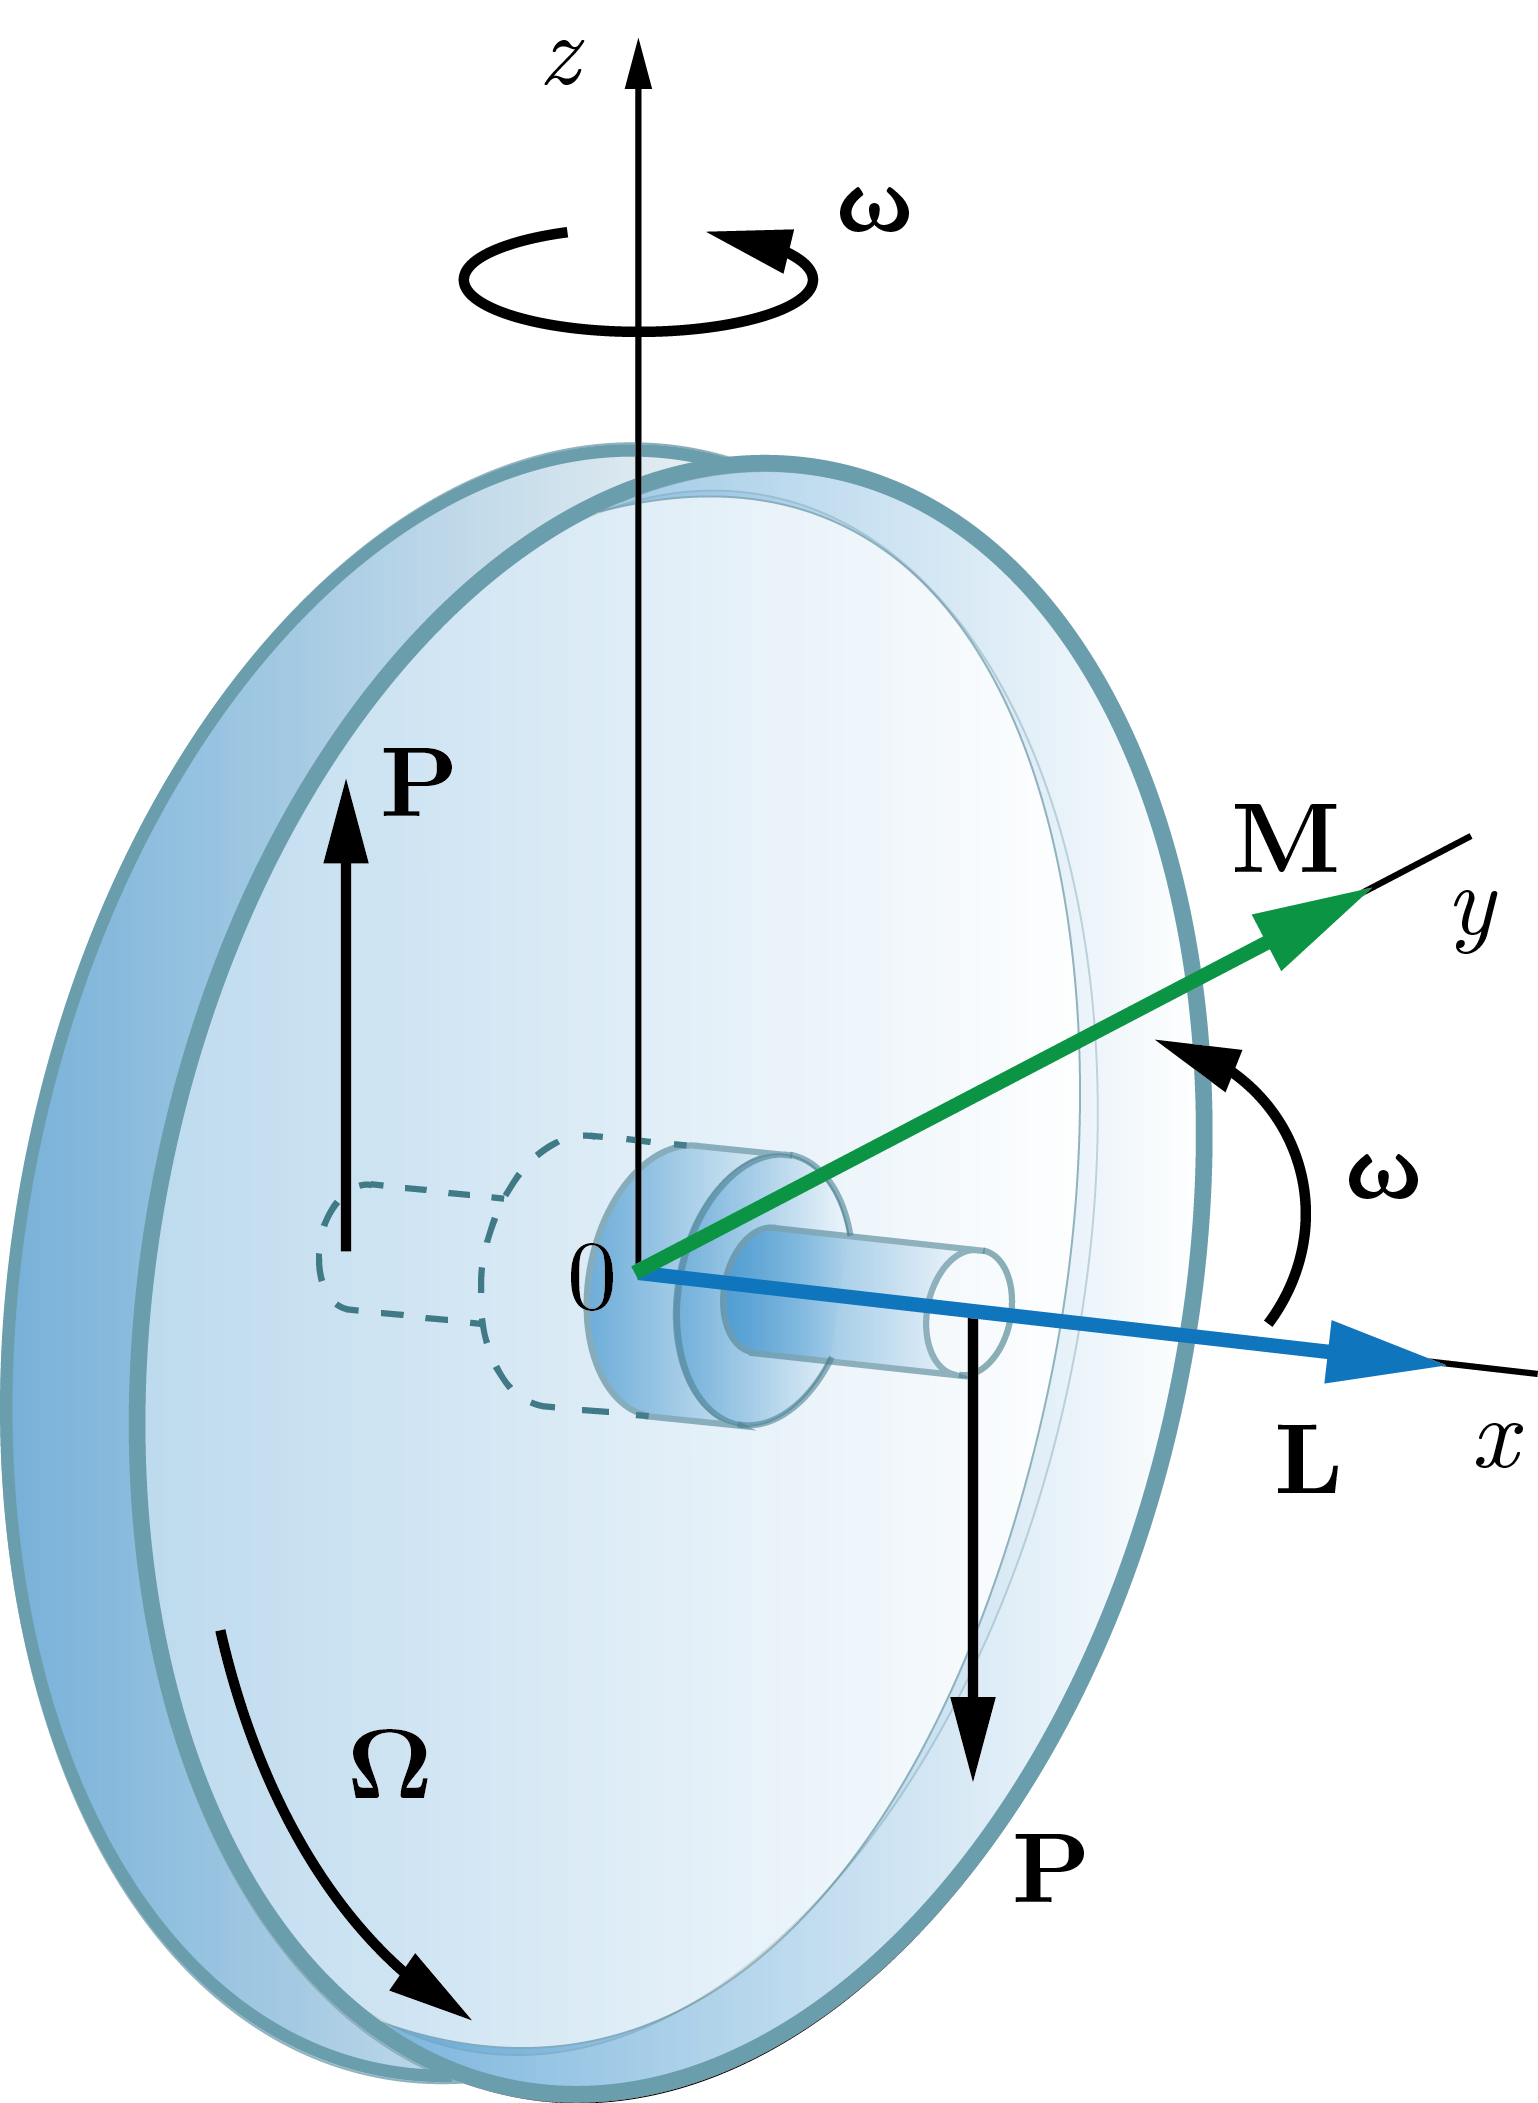
\includegraphics[width=0.45\linewidth]{chair-3.png}
	\caption{Опыт с быстро вращающимся гироскопом. Чтобы повернуть ось гироскопа в горизонтальной плоскости, следует надавить на нее левой рукой вниз, а правой - вверх}
	\label{chair-3}
\end{figure}

Согласно правилу прецессии, движение оси $x$ собственного вращения колеса должно происходить так, если бы вектор \textbf{L} стремился к совмещению с вектором \textbf{М} по кратчайшему пути.
В результате и будет наблюдаться прецессия оси гироскопа в горизонтальной плоскости с угловой скоростью $ \omega $, указанной на рис.\ref{chair-eq3}.
Нетрудно убедиться в том, что если попытаться повернуть ось вращающегося колеса в горизонтальной плоскости, то на самом деле эта ось будет поворачиваться в плоскости вертикальной.
\newpage

\textit{Опыт 3}:
Человек, стоящий на неподвижной скамье, получает, вращающийся вокруг вертикальной оси (рис.\ref{chair-2},\textit{в}), диск гироскопа. 
В этом случае момент импульса системы человек и платформа-колесо определяется только моментом импульса колеса:
\begin{equation}\label{chair-eq8}
L = I_{0} \dot 0 + I_{\text{д}}\bm{\omega}_{\text{д}} = I_{\text{д}}\bm{\omega}_{\text{д}},
\end{equation}
где $ I_{0} $ — момент инерции человека и платформы; $ I_{\text{д}} $ и $ \bm{\omega}_{\text{д}} $ — момент инерции и угловая скорость диска гироскопа.
Так как момент внешних сил относительно вертикальной оси равен нулю, то $ L $ сохраняется ($ L = \text{const} $).
Если повернуть ось вращения колеса на 180° (рис.\ref{chair-2},\textit{г}), то момент импульса колеса будет направлен противоположно первоначальному и равен $ I_{\text{д}}\bm{\omega}_{\text{д}} $.
Так как вектор момента импульса колеса изменяется, а момент импульса системы сохраняется, то неизбежно должен измениться и момент импульса, человека и платформы, он уже не будет равен нулю (тут можно пренебречь небольшим несовпадением оси вращения платформы с осью вращения диска ).
Момент импульса системы в этом случае:
\begin{equation}\label{chair-eq9}
L = I_{0}\bm{\omega}_{0} + (- I_{\text{д}}\bm{\omega}_{\text{д}}).
\end{equation}
Из закона сохранения момента импульса позволяет приравнять выражения (\ref{chair-eq8}) и (\ref{chair-eq9}):
\begin{equation}\label{chair-eq10}
I_{\text{д}}\bm{\omega}_{\text{д}} = I_{0}\bm{\omega}_{0} + (- I_{\text{д}}\bm{\omega}_{\text{д}}).
\end{equation}
Или в скалярной форме:
\begin{equation}\label{chair-eq11}
I_{\text{д}}\omega_{\text{д}} = I_{0}\omega_{0} + (- I_{\text{д}}\omega_{\text{д}}).
\end{equation}
Преобразуем уравнение (\ref{chair-eq11})
\begin{equation}\label{chair-eq12}
I_{0}\omega_{0} =  2I_{\text{д}}\omega_{\text{д}}.
\end{equation}
Из уравнения (\ref{chair-eq12}) можно к примеру приближенно оценить момент инерции тела человека вместе с платформой, для чего необходимо измерить $ \omega_{\text{д}} $, $ \omega_{0} $ и найти $ I_{\text{д}} $.

\end{document}
	
